% 荷质比的测定
%汤姆孙测电子荷质比的方法|磁聚焦法

\pentry{静电的基本规律和性质\upref{EM1}}

\subsection{荷质比}
原理:利用电子(或其他带电粒子)在磁场中偏转性的特点,测得粒子电荷与质量之比(即荷质比)
说明:荷质比是带电微观粒子的基本参量之一.

典型的测量荷质比的方式有两种

\subsection{汤姆孙测量电子荷质比的方法}

\begin{figure}[ht]
\centering
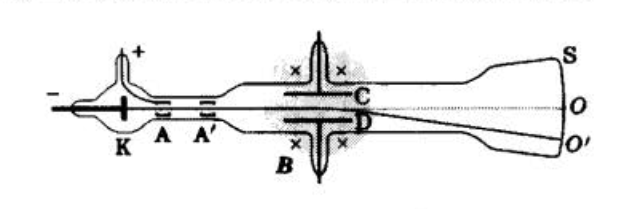
\includegraphics[width=7cm]{./figures/Charge_1.png}
\caption{汤姆孙法测荷质比} \label{Charge_fig1}
\end{figure}

玻璃管内抽成真空,在阳极$A$与阴极$K$之间维持数千伏特的电压,靠管内残存的气体的离子在阴极引起的二次发射产生电子流.阳极$A$和第二个金属屏$A'$中央各有一个小孔,$K$、$A$之间被加速了电子流,只有很窄一束能够通过两孔.玻璃管的中部$C$、$D$为电容板的两极板,在其间可产生一竖直方向的电场.图中阴影部分,是由管外的电磁铁产生一方向垂直纸面的磁场.适当的调节电场和磁场的强度,可使它们作用在电子上的力达到平衡,即:
\begin{equation}
eE=evB
\end{equation}

然后,将电场切断,电子束在磁场区域内将沿圆弧运动,此圆弧半径可得:
\begin{equation}
R=\frac {mv}{eB}
\end{equation}

因此,电子的荷质比为:
\begin{equation}
\frac{e}{m}=\frac{v}{RB}=\frac {E}{RB^2}
\end{equation}
通过测得$R$之后,我们就能求出荷质比了.

\subsection{磁聚焦法}

\begin{figure}[ht]
\centering
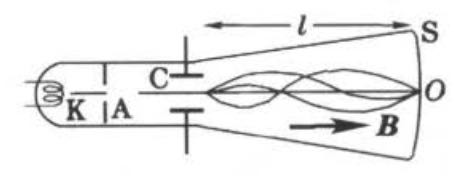
\includegraphics[width=7cm]{./figures/Charge_2.png}
\caption{磁聚焦法测荷质比} \label{Charge_fig2}
\end{figure}

抽真空的玻璃管中装有热阴极K和有小孔的阳极 $A$.在 $A$,$K$ 之间加电压 $\Delta U$ 时,由阳极的小孔射出的电子动能为:
\begin{equation}
\frac{1}{2mv^2}=e\Delta U
\end{equation}

从得到其速率为:
\begin{equation}
v=\sqrt{\frac{2e\Delta U}{m}}
\end{equation}
在电容器 $C$ 上加一个不大的横向交变电场,使不同时刻通过这里的电子发生不同程度的偏转.在电容器 $C$ 和荧光屏 $S$ 之间加一均匀的纵向磁场,电子从$C$出来后将沿螺旋线运动,到达距离$h=\frac{2\pi mv}{eB}$的地方聚焦.适当的调节磁感应强度$B$大小,使得电子流的焦点落在荧光屏$S$上.其中$h$是$C$到$S$间的距离.将上述方程中的$v$消去,我们有:
\begin{equation}
\frac {e}{m}=\frac{8\pi ^2 \Delta U}{h^2 B^2}
\end{equation}
(上式中方程右边的各量都能够测出来,因此我们能够确定$e/m$)


参考文献:赵凯华, 陈熙谋. 电磁学[M]. Gao deng jiao yu chu ban she, 2011.
